\documentclass[11pt, letterpaper]{article}
\usepackage[margin=0.5in]{geometry}
\usepackage{graphicx}

\begin{document}

\title{String Search}
\author{Drew Aparicio}
\date{February 20, 2025}
\maketitle

\section{Introduction}
An organism's DNA encompasses all instructions for its development and
function. To link specific DNA sequences to particular traits or diseases, we
analyze the DNA of individuals exhibiting similar or differing characteristics.
DNA's structure—a long sequence of nucleotides denoted by A, C, T, and
G—transforms the comparison of two genomes into a computational string search
challenge. This problem involves two input strings: a typically longer string,
the text $T$, and a usually shorter string, the pattern $P$. The
objective is to locate every instance of $P$ within $T$. Here we compare the
the efficiency and memory consumption between two string search algorithms that
align $P$ with all possible positions in $T$. The more simple algorithm had a faster runtime for text sizes below three times the pattern size (held constant here), but the more complex algorithm had faster runtimes for all text sizes more than three times the size of the pattern. So, for situations where the pattern is much shorter than the text (often in genomics), the more complex Boyer-Moore algorithm should be used for searching. 

Additionally, when text size is held constant, an increase in $P$ will lead to a decrease in runtime for the simple algorithm and a much larger increase in runtime for the complex algorithm. Similarly, the memory usage for the simple algorithm stays relatively low, whereas that of the complex algorithm increases in a step-wise pattern (due to dynamic memory allocation).

Finally, for a worst-case scenario, the Naive Search will outperform the Boyer-Moore search in runtime by about 2 times, but it's memory usage is much larger than that of Boyer-Moore. So, for cases similar to this, it may be useful to implement a Naive Search for maximal efficiency.

\section{Results}

As expected when $P$ is constant, the runtime of the naive string search algorithm increased
linearly and the memory usage remained constant as the text size increased. However, for the Boyer-Moore search algorithm, the runtime stayed relatively constant with an increase in text sizes, outperforming the naive search once the text size surpassed about three times the pattern size. The trade-off, however, is that the Boyer-Moore search constantly used much more memory than the naive search.
(Figure~\ref{timeandmem}). 

For naive search, the algorithm's runtime increased linearly with
the text size because the algorithm considers all possible alignments of the
pattern $P$ with the text $T$. As the text size increases, the number of
possible alignments increases linearly. The algorithm's memory usage remained
constant because the algorithm only stores the positions of the pattern $P$ in
the text $T$. 

For Boyer-Moore, the algorithm's runtime remained relatively constant with the text size because with a unique pattern (not appearing often in a large text), the algorithm can make large jumps to efficiently skip over many parts of the text that do not contain the pattern. This graph demonstrates how Boyer-Moore string search very closely exhibits $\mathcal{O}(n/m)$ runtime, where $n$ is the text size and $m$ is the pattern size. The algorithm's memory usage remained constant, but much higher than that of naive search, because the algorithm stores both the bad character table and the good suffix table of the pattern, which remained at a constant size.

\begin{figure}[ht] \centering
    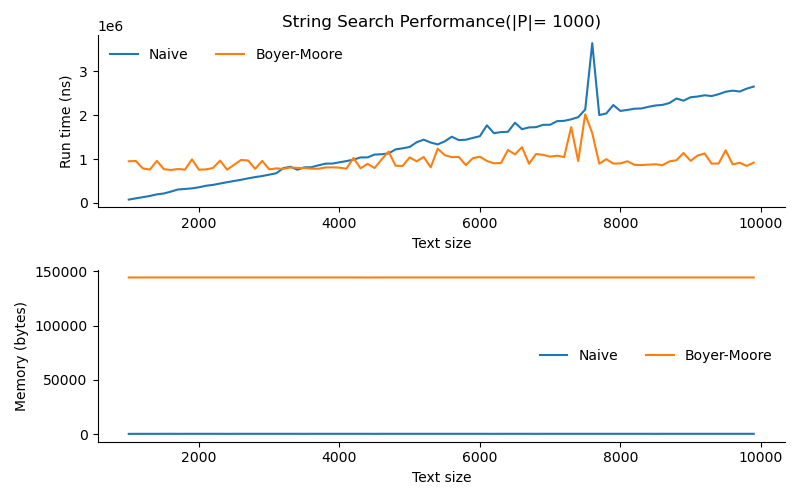
\includegraphics[width=0.6\textwidth]{t-range_p-1000.png}
    \caption{The empirical runtime and memory usage of the naive and Boyer-Moore string search
    algorithms considering a pattern size of 1000 and a database size ranging
    from 1000 to 10,000 characters.}
    \label{timeandmem}
\end{figure}

\newpage

When $T$ is constant, the runtimes exhibit similar behaviors: naive search performs better when the text size is below three times the pattern size (pattern size is above 1/3 of the text size) as seen in Figure \ref{timeandmem2}. For memory usage, the naive search, once again, stayed constant at a low value. However, the Boyer-Moore search increased in a step-wise way as the length of the pattern increased. This step-wise increase can be attributed to the dynamic memory allocation of the program, which allocated double the amount of memory once a threshold amount of memory was used. In other words, as the pattern size increased, the program had to continue doubling the memory to be used until it could accommodate all of the memory needed for the bad character and good suffix tables.\\\\

\begin{figure}[ht] \centering
    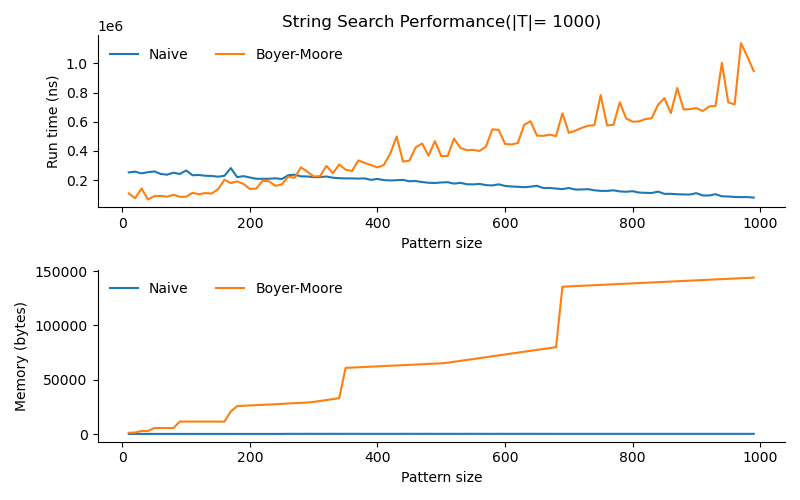
\includegraphics[width=0.6\textwidth]{t-1000_p-range.png}
    \caption{The empirical runtime and memory usage of the naive and Boyer-Moore string search
    algorithms considering a database size of 1000 and a pattern size ranging
    from 10 to 1,000 characters.}
    \label{timeandmem2}
\end{figure}

Finally, when analyzing a worst-case scenario, where the pattern appears at every index of the pattern, the naive search outperformed the Boyer-Moore search by two times in terms of runtime. The naive search took an average of 6610.3 ns, whereas the Boyer-Moore search took an average of 10306.9 ns. This extra processing time comes from the fact that the Boyer-Moore search has to preprocess the pattern and determine the shift it needs to make (will always be 1) every iteration, whereas the naive search immediately shifts 1.


\section{Methods}

\subsection{Naive string search}
The naive string search algorithm considers all possible alignments of the
pattern $P$ with the text $T$. Staring at the first position in $T$, the
algorithm compares $P$'s characters with the corresponding characters in $T$.
If all characters match, the algorithm records the alignment's position in $T$.
The algorithm then repeats this process for the next alignment. If any of the 
characters in $P$ do not match a corresponding character in $T$, the current
alignment breaks and then $P$ shifts down one position in $T$, and the process
repeats. This process continues until $P$ has been compared to all possible
alignments in $T$, then returns the recorded positions.

\subsection{Boyer-Moore string search}
The Boyer-Moore string search algorithm uses two tables of predetermined shifts to efficiently skip over sections of the text while still finding all possible occurrences of the
pattern $P$ within the text $T$. The algorithm preprocesses the pattern to create the bad character and good suffix tables, which will determine the next shift based on the mismatched character in $T$ or the position in $P$ where the mismatch happened, respectively. At each shift, $P$ is compared with $T$ starting from the end of $P$ until a mismatch is found, at which point the algorithm will shift based on the max value returned from the bad character table and the good suffix table.
The returned shift value from the bad character table shifts the pattern so that the last occurrence of the mismatched character in the pattern aligns with its occurrence in the text. For the good suffix table, if a suffix of the pattern matches in $T$ but the mismatch occurs earlier in $P$, the returned shift value will shift the pattern to align with the next occurrence of the matching suffix. If no mismatch is found, the algorithm will note this index in $T$ as an occurrence of $P$ and will shift the pattern down the text by 1. This process continues until the shift value is greater than the length of $T$ minus the length of $P$ ($P$ has been shifted beyond the end of $T$).

\subsection{Empirical comparison}

We evaluated the performance of the naive and Boyer-Moore string search algorithms considering a
pattern size of 1000 and text sizes that ranged from 1000 to 10,000 characters
with a step size of 100. Additionally, we evaluated the performance of these algorithms considering a text size of 1000 and pattern sizes that ranged from 10 to 1000 characters with a step size of 10.
For both evaluations, the performance metrics include runtime and memory
usage. For each text size, we ran a single search where we generated a random
string for $T$ from the alphabet ${A, C, T, G}$ and extracted a random
substring $P$ from $T$. We then recorded the runtime and memory usage of the
algorithm consiuder that $P$ and $T$. After the round was complete for a given
text size, we calculated the average runtime and memory usage for the search.

For the worst-case scenario, we evaluated the same performance metrics (average runtime and memory usage over 10 rounds) considering the given text size of 20 and the given pattern size of 20, where the pattern matched at every position in the text.

\subsection{Reproducibility}
To replicate the first experiment (constant pattern size), clone the repository and then run the
following commands from the root directory of the repository:
\begin{verbatim}
$ git clone https://github.com/cu-compg-spring-2025/assignment-4-string-search-drewapar.git
$ cd assignment-4-string-search-drewapar
$ python src/string_search.py \
    --text_range 1000 10000 100 \
    --pattern_range 1000 1000 1000 \
    --rounds 1 \
    --out_file doc/t-range_p-1000.png
\end{verbatim}
%%%% Add your command here%%%%


\noindent To replicate the second experiment (constant text size), run the following command:
\begin{verbatim}
$ python src/string_search.py \
    --text_range 1000 1000 1000 \
    --pattern_range 10 1000 10 \
    --rounds 1 \
    --out_file doc/t-1000_p-range.png
\end{verbatim}


\noindent Finally, to replicate the worst-case experiment, run the following command:
\begin{verbatim}
$ python src/test_string_search.py \
    --text 'AAAAAAAAAAAAAAAAAAAA' \
    --pattern 'AA' \
    --rounds 10 
\end{verbatim}
Which will produce the output:
\begin{verbatim}
Naive Search average runtime: [6610.3]
Naive Search average memory usage: [144.0]
Boyer-Moore average runtime: [10306.9]
Boyer-Moore average memory usage: [0.0]
\end{verbatim}

\end{document}
